\newpage

\section{Messwerte}
\label{sec:Messwerte}

\subsection{Schallgeschwindigkeitsbestimmung mit dem Impuls-Echo-Verfahren}

    \begin{figure}
        \centering
        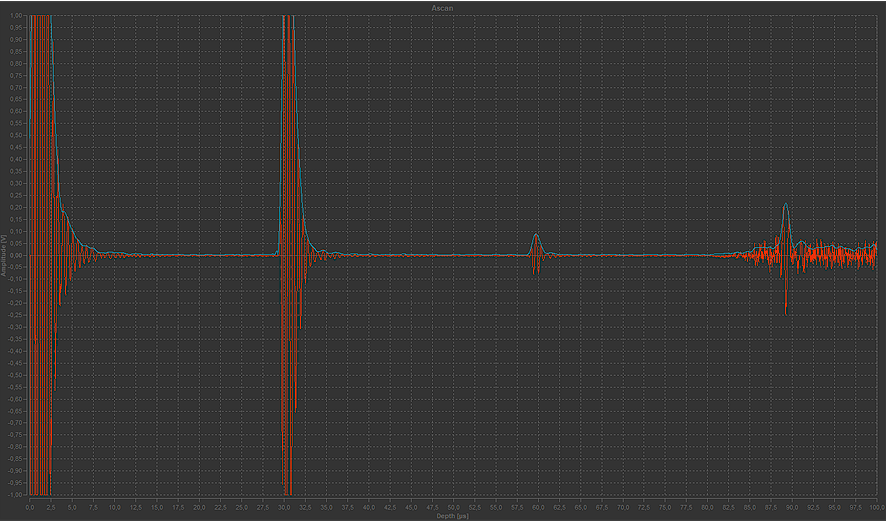
\includegraphics[width=15cm]{messwerte/Impuls-Echo/4_ImEc.png}
        \caption{A-Scan des 4 cm hohen Zylinders mittels Echo-Impuls.}
    \end{figure}

    \begin{figure}
        \centering
        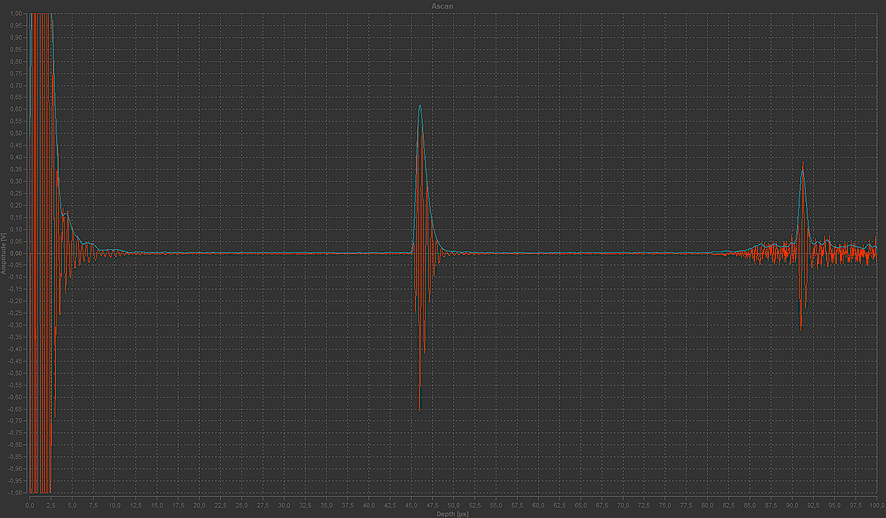
\includegraphics[width=15cm]{messwerte/Impuls-Echo/6_ImEc.png}
        \caption{A-Scan des 6 cm hohen Zylinders mittels Echo-Impuls.}
    \end{figure}

    \begin{figure}
        \centering
        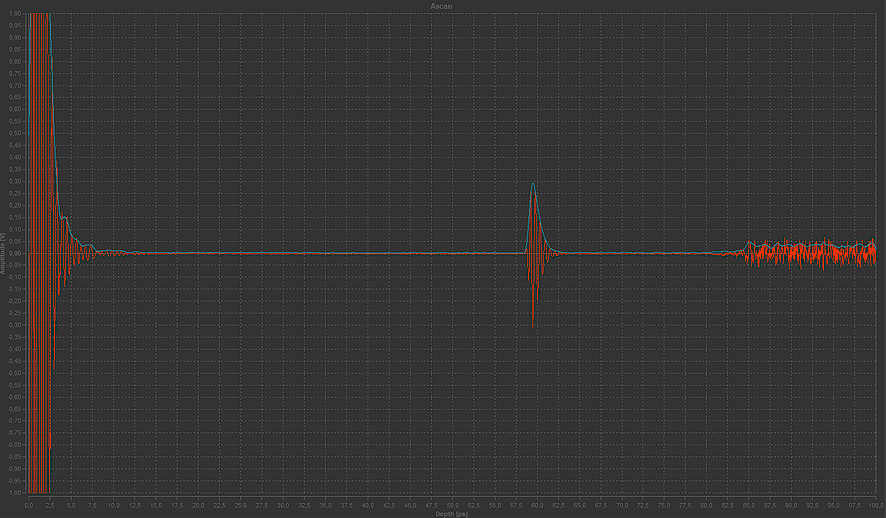
\includegraphics[width=15cm]{messwerte/Impuls-Echo/8_ImEc.png}
        \caption{A-Scan des 8 cm hohen Zylinders mittels Echo-Impuls.}
    \end{figure}

    \begin{figure}
        \centering
        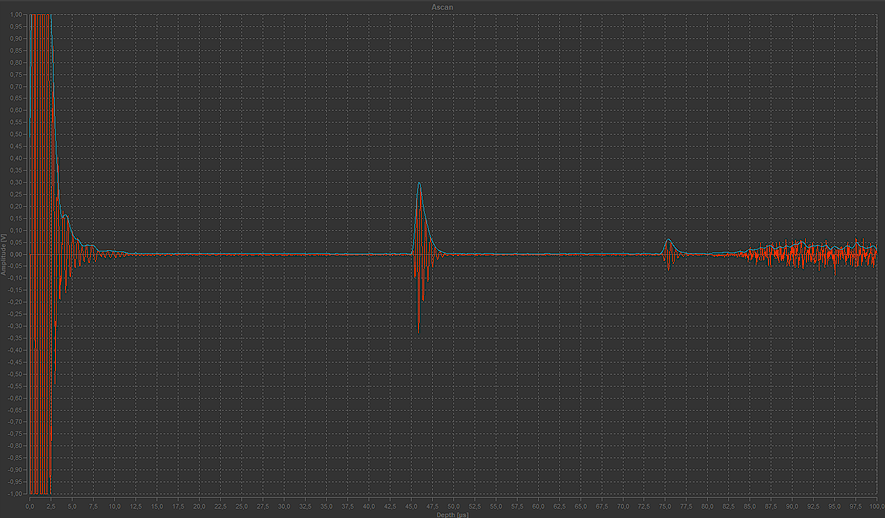
\includegraphics[width=15cm]{messwerte/Impuls-Echo/10_ImEc.png}
        \caption{A-Scan des zusammengesetzten 10 cm hohen Zylinders mittels Echo-Impuls.}
    \end{figure}

    \begin{figure}
        \centering
        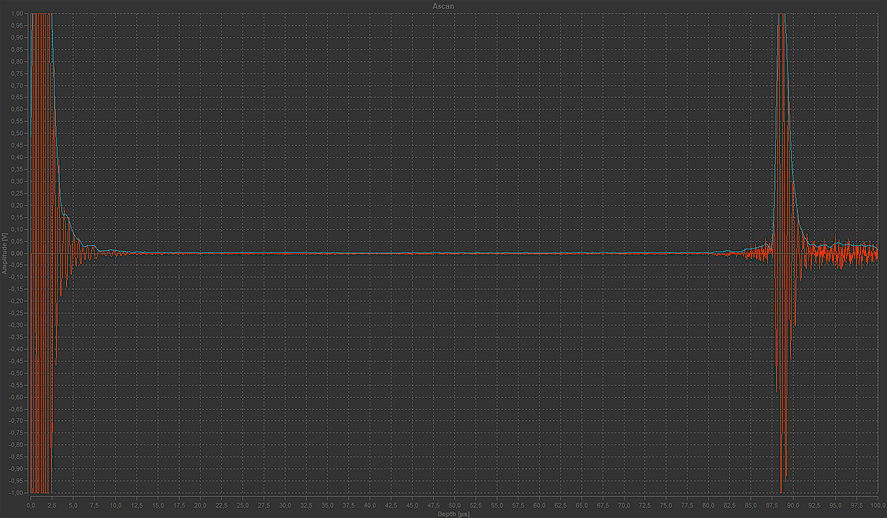
\includegraphics[width=15cm]{messwerte/Impuls-Echo/12_ImEc.png}
        \caption{A-Scan des 12 cm hohen Zylinders mittels Echo-Impuls.}
    \end{figure}

\subsection{Schallgeschwindigkeitsbestimmung mit Durchschallungs-Verfahren}

    \begin{figure}
        \centering
        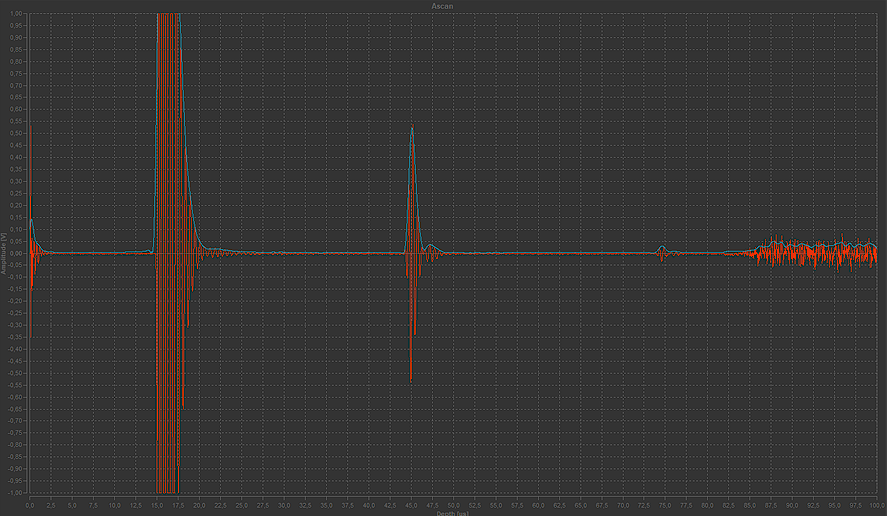
\includegraphics[width=15cm]{messwerte/Durchschallung/4_Durch.png}
        \caption{A-Scan des 4 cm hohen Zylinders mittels Durchschallung.}
    \end{figure}

    \begin{figure}
        \centering
        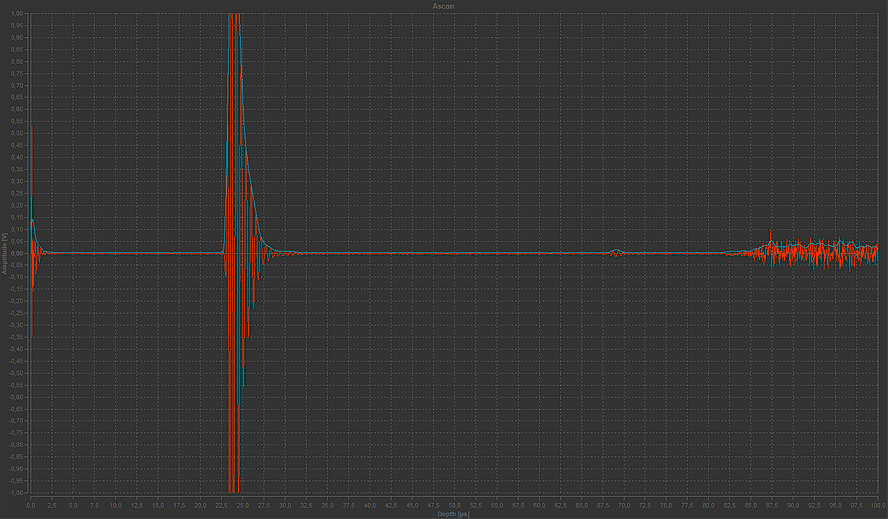
\includegraphics[width=15cm]{messwerte/Durchschallung/6_Durch.png}
        \caption{A-Scan des 6 cm hohen Zylinders mittels Durchschallung.}
    \end{figure}

    \begin{figure}
        \centering
        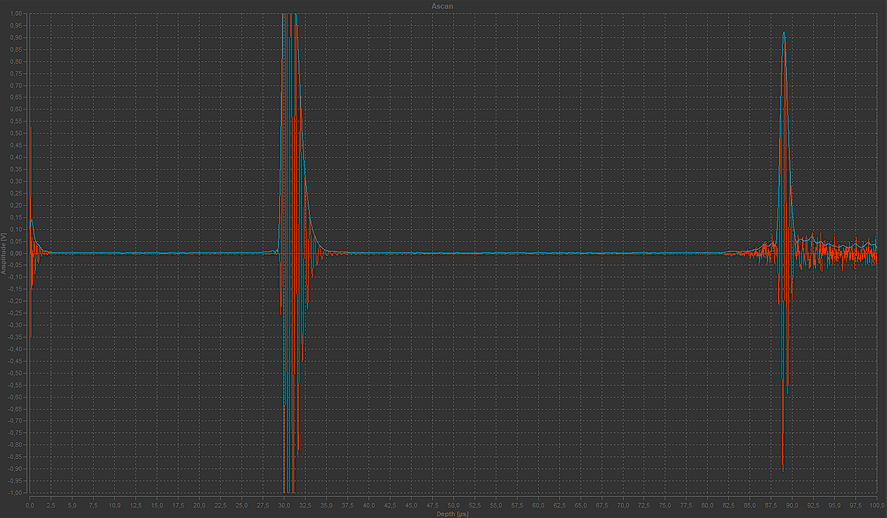
\includegraphics[width=15cm]{messwerte/Durchschallung/8_Durch.png}
        \caption{A-Scan des 8 cm hohen Zylinders mittels Durchschallung.}
    \end{figure}

    \begin{figure}
        \centering
        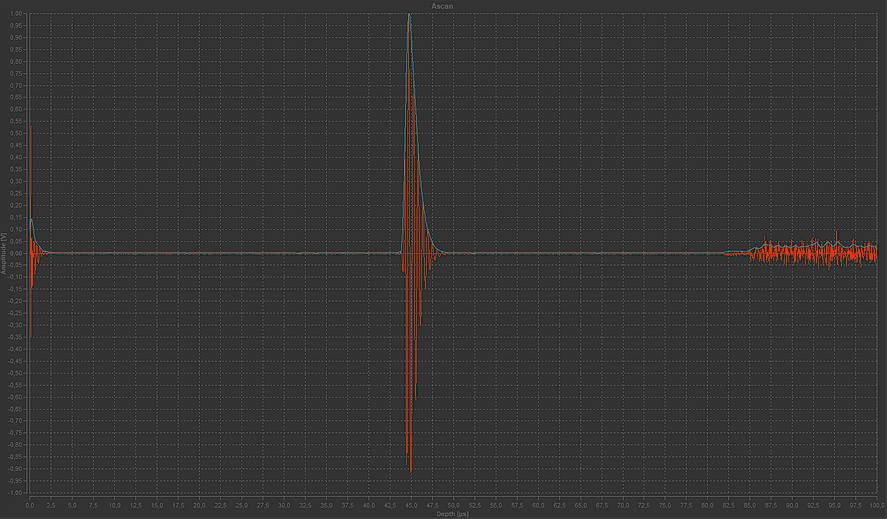
\includegraphics[width=15cm]{messwerte/Durchschallung/12_Durch.png}
        \caption{A-Scan des 12 cm hohen Zylinders mittels Durchschallung.}
    \end{figure}

\subsection{Biometrische Untersuchung eines Augenmodells}

    \begin{figure}
        \centering
        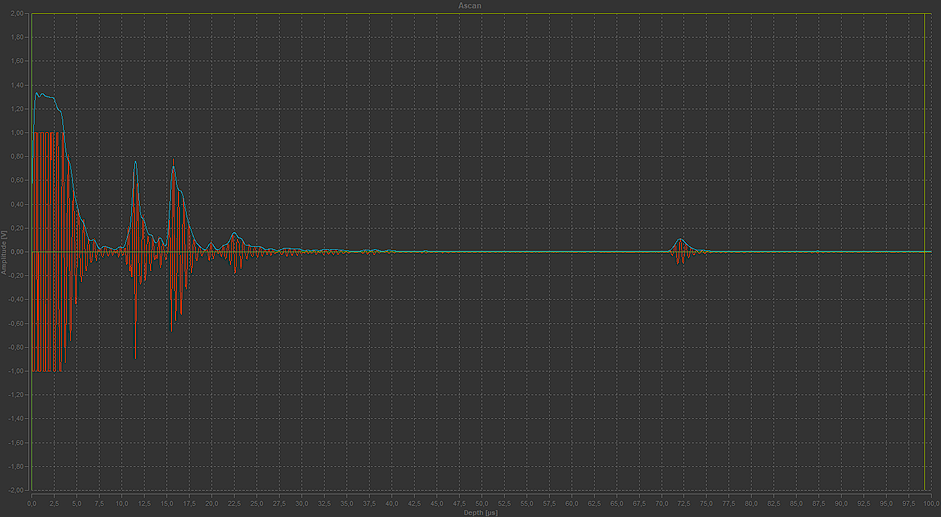
\includegraphics[width=15cm]{messwerte/Durchschallung/Auge.png}
        \caption{A-Scan des Augenmodells mittels Echo-Impuls.}
    \end{figure}